
%% bare_conf.tex
%% V1.4b
%% 2015/08/26
%% by Michael Shell
%% See:
%% http://www.michaelshell.org/
%% for current contact information.
%%
%% This is a skeleton file demonstrating the use of IEEEtran.cls
%% (requires IEEEtran.cls version 1.8b or later) with an IEEE
%% conference paper.
%%
%% Support sites:
%% http://www.michaelshell.org/tex/ieeetran/
%% http://www.ctan.org/pkg/ieeetran
%% and
%% http://www.ieee.org/

%%*************************************************************************
%% Legal Notice:
%% This code is offered as-is without any warranty either expressed or
%% implied; without even the implied warranty of MERCHANTABILITY or
%% FITNESS FOR A PARTICULAR PURPOSE! 
%% User assumes all risk.
%% In no event shall the IEEE or any contributor to this code be liable for
%% any damages or losses, including, but not limited to, incidental,
%% consequential, or any other damages, resulting from the use or misuse
%% of any information contained here.
%%
%% All comments are the opinions of their respective authors and are not
%% necessarily endorsed by the IEEE.
%%
%% This work is distributed under the LaTeX Project Public License (LPPL)
%% ( http://www.latex-project.org/ ) version 1.3, and may be freely used,
%% distributed and modified. A copy of the LPPL, version 1.3, is included
%% in the base LaTeX documentation of all distributions of LaTeX released
%% 2003/12/01 or later.
%% Retain all contribution notices and credits.
%% ** Modified files should be clearly indicated as such, including  **
%% ** renaming them and changing author support contact information. **
%%*************************************************************************


% *** Authors should verify (and, if needed, correct) their LaTeX system  ***
% *** with the testflow diagnostic prior to trusting their LaTeX platform ***
% *** with production work. The IEEE's font choices and paper sizes can   ***
% *** trigger bugs that do not appear when using other class files.       ***                          ***
% The testflow support page is at:
% http://www.michaelshell.org/tex/testflow/



\documentclass[conference]{IEEEtran}
% Some Computer Society conferences also require the compsoc mode option,
% but others use the standard conference format.
%
% If IEEEtran.cls has not been installed into the LaTeX system files,
% manually specify the path to it like:
% \documentclass[conference]{../sty/IEEEtran}
\usepackage{graphicx}




% Some very useful LaTeX packages include:
% (uncomment the ones you want to load)


% *** MISC UTILITY PACKAGES ***
%
%\usepackage{ifpdf}
% Heiko Oberdiek's ifpdf.sty is very useful if you need conditional
% compilation based on whether the output is pdf or dvi.
% usage:
% \ifpdf
%   % pdf code
% \else
%   % dvi code
% \fi
% The latest version of ifpdf.sty can be obtained from:
% http://www.ctan.org/pkg/ifpdf
% Also, note that IEEEtran.cls V1.7 and later provides a builtin
% \ifCLASSINFOpdf conditional that works the same way.
% When switching from latex to pdflatex and vice-versa, the compiler may
% have to be run twice to clear warning/error messages.






% *** CITATION PACKAGES ***
%
%\usepackage{cite}
% cite.sty was written by Donald Arseneau
% V1.6 and later of IEEEtran pre-defines the format of the cite.sty package
% \cite{} output to follow that of the IEEE. Loading the cite package will
% result in citation numbers being automatically sorted and properly
% "compressed/ranged". e.g., [1], [9], [2], [7], [5], [6] without using
% cite.sty will become [1], [2], [5]--[7], [9] using cite.sty. cite.sty's
% \cite will automatically add leading space, if needed. Use cite.sty's
% noadjust option (cite.sty V3.8 and later) if you want to turn this off
% such as if a citation ever needs to be enclosed in parenthesis.
% cite.sty is already installed on most LaTeX systems. Be sure and use
% version 5.0 (2009-03-20) and later if using hyperref.sty.
% The latest version can be obtained at:
% http://www.ctan.org/pkg/cite
% The documentation is contained in the cite.sty file itself.






% *** GRAPHICS RELATED PACKAGES ***
%
\ifCLASSINFOpdf
  % \usepackage[pdftex]{graphicx}
  % declare the path(s) where your graphic files are
  % \graphicspath{{../pdf/}{../jpeg/}}
  % and their extensions so you won't have to specify these with
  % every instance of \includegraphics
  % \DeclareGraphicsExtensions{.pdf,.jpeg,.png}
\else
  % or other class option (dvipsone, dvipdf, if not using dvips). graphicx
  % will default to the driver specified in the system graphics.cfg if no
  % driver is specified.
  % \usepackage[dvips]{graphicx}
  % declare the path(s) where your graphic files are
  % \graphicspath{{../eps/}}
  % and their extensions so you won't have to specify these with
  % every instance of \includegraphics
  % \DeclareGraphicsExtensions{.eps}
\fi
% graphicx was written by David Carlisle and Sebastian Rahtz. It is
% required if you want graphics, photos, etc. graphicx.sty is already
% installed on most LaTeX systems. The latest version and documentation
% can be obtained at: 
% http://www.ctan.org/pkg/graphicx
% Another good source of documentation is "Using Imported Graphics in
% LaTeX2e" by Keith Reckdahl which can be found at:
% http://www.ctan.org/pkg/epslatex
%
% latex, and pdflatex in dvi mode, support graphics in encapsulated
% postscript (.eps) format. pdflatex in pdf mode supports graphics
% in .pdf, .jpeg, .png and .mps (metapost) formats. Users should ensure
% that all non-photo figures use a vector format (.eps, .pdf, .mps) and
% not a bitmapped formats (.jpeg, .png). The IEEE frowns on bitmapped formats
% which can result in "jaggedy"/blurry rendering of lines and letters as
% well as large increases in file sizes.
%
% You can find documentation about the pdfTeX application at:
% http://www.tug.org/applications/pdftex





% *** MATH PACKAGES ***
%
\usepackage{amsmath}
\usepackage{amssymb}
\DeclareMathOperator*{\argmin}{arg\,min}
\DeclareMathOperator*{\argmax}{arg\,max}
% A popular package from the American Mathematical Society that provides
% many useful and powerful commands for dealing with mathematics.
%
% Note that the amsmath package sets \interdisplaylinepenalty to 10000
% thus preventing page breaks from occurring within multiline equations. Use:
%\interdisplaylinepenalty=2500
% after loading amsmath to restore such page breaks as IEEEtran.cls normally
% does. amsmath.sty is already installed on most LaTeX systems. The latest
% version and documentation can be obtained at:
% http://www.ctan.org/pkg/amsmath





% *** SPECIALIZED LIST PACKAGES ***
%
%\usepackage{algorithmic}
% algorithmic.sty was written by Peter Williams and Rogerio Brito.
% This package provides an algorithmic environment fo describing algorithms.
% You can use the algorithmic environment in-text or within a figure
% environment to provide for a floating algorithm. Do NOT use the algorithm
% floating environment provided by algorithm.sty (by the same authors) or
% algorithm2e.sty (by Christophe Fiorio) as the IEEE does not use dedicated
% algorithm float types and packages that provide these will not provide
% correct IEEE style captions. The latest version and documentation of
% algorithmic.sty can be obtained at:
% http://www.ctan.org/pkg/algorithms
% Also of interest may be the (relatively newer and more customizable)
% algorithmicx.sty package by Szasz Janos:
% http://www.ctan.org/pkg/algorithmicx




% *** ALIGNMENT PACKAGES ***
%
%\usepackage{array}
% Frank Mittelbach's and David Carlisle's array.sty patches and improves
% the standard LaTeX2e array and tabular environments to provide better
% appearance and additional user controls. As the default LaTeX2e table
% generation code is lacking to the point of almost being broken with
% respect to the quality of the end results, all users are strongly
% advised to use an enhanced (at the very least that provided by array.sty)
% set of table tools. array.sty is already installed on most systems. The
% latest version and documentation can be obtained at:
% http://www.ctan.org/pkg/array


% IEEEtran contains the IEEEeqnarray family of commands that can be used to
% generate multiline equations as well as matrices, tables, etc., of high
% quality.




% *** SUBFIGURE PACKAGES ***
%\ifCLASSOPTIONcompsoc
%  \usepackage[caption=false,font=normalsize,labelfont=sf,textfont=sf]{subfig}
%\else
%  \usepackage[caption=false,font=footnotesize]{subfig}
%\fi
% subfig.sty, written by Steven Douglas Cochran, is the modern replacement
% for subfigure.sty, the latter of which is no longer maintained and is
% incompatible with some LaTeX packages including fixltx2e. However,
% subfig.sty requires and automatically loads Axel Sommerfeldt's caption.sty
% which will override IEEEtran.cls' handling of captions and this will result
% in non-IEEE style figure/table captions. To prevent this problem, be sure
% and invoke subfig.sty's "caption=false" package option (available since
% subfig.sty version 1.3, 2005/06/28) as this is will preserve IEEEtran.cls
% handling of captions.
% Note that the Computer Society format requires a larger sans serif font
% than the serif footnote size font used in traditional IEEE formatting
% and thus the need to invoke different subfig.sty package options depending
% on whether compsoc mode has been enabled.
%
% The latest version and documentation of subfig.sty can be obtained at:
% http://www.ctan.org/pkg/subfig




% *** FLOAT PACKAGES ***
%
%\usepackage{fixltx2e}
% fixltx2e, the successor to the earlier fix2col.sty, was written by
% Frank Mittelbach and David Carlisle. This package corrects a few problems
% in the LaTeX2e kernel, the most notable of which is that in current
% LaTeX2e releases, the ordering of single and double column floats is not
% guaranteed to be preserved. Thus, an unpatched LaTeX2e can allow a
% single column figure to be placed prior to an earlier double column
% figure.
% Be aware that LaTeX2e kernels dated 2015 and later have fixltx2e.sty's
% corrections already built into the system in which case a warning will
% be issued if an attempt is made to load fixltx2e.sty as it is no longer
% needed.
% The latest version and documentation can be found at:
% http://www.ctan.org/pkg/fixltx2e


%\usepackage{stfloats}
% stfloats.sty was written by Sigitas Tolusis. This package gives LaTeX2e
% the ability to do double column floats at the bottom of the page as well
% as the top. (e.g., "\begin{figure*}[!b]" is not normally possible in
% LaTeX2e). It also provides a command:
%\fnbelowfloat
% to enable the placement of footnotes below bottom floats (the standard
% LaTeX2e kernel puts them above bottom floats). This is an invasive package
% which rewrites many portions of the LaTeX2e float routines. It may not work
% with other packages that modify the LaTeX2e float routines. The latest
% version and documentation can be obtained at:
% http://www.ctan.org/pkg/stfloats
% Do not use the stfloats baselinefloat ability as the IEEE does not allow
% \baselineskip to stretch. Authors submitting work to the IEEE should note
% that the IEEE rarely uses double column equations and that authors should try
% to avoid such use. Do not be tempted to use the cuted.sty or midfloat.sty
% packages (also by Sigitas Tolusis) as the IEEE does not format its papers in
% such ways.
% Do not attempt to use stfloats with fixltx2e as they are incompatible.
% Instead, use Morten Hogholm'a dblfloatfix which combines the features
% of both fixltx2e and stfloats:
%
% \usepackage{dblfloatfix}
% The latest version can be found at:
% http://www.ctan.org/pkg/dblfloatfix


% *** PDF, URL AND HYPERLINK PACKAGES ***
%
%\usepackage{url}
% url.sty was written by Donald Arseneau. It provides better support for
% handling and breaking URLs. url.sty is already installed on most LaTeX
% systems. The latest version and documentation can be obtained at:
% http://www.ctan.org/pkg/url
% Basically, \url{my_url_here}.




% *** Do not adjust lengths that control margins, column widths, etc. ***
% *** Do not use packages that alter fonts (such as pslatex).         ***
% There should be no need to do such things with IEEEtran.cls V1.6 and later.
% (Unless specifically asked to do so by the journal or conference you plan
% to submit to, of course. )


% correct bad hyphenation here
\hyphenation{op-tical net-works semi-conduc-tor}

\begin{document}
%
% paper title
% Titles are generally capitalized except for words such as a, an, and, as,
% at, but, by, for, in, nor, of, on, or, the, to and up, which are usually
% not capitalized unless they are the first or last word of the title.
% Linebreaks \\ can be used within to get better formatting as desired.
% Do not put math or special symbols in the title.
\title{COMS 4771 Kaggle Competition Report\\ from Deus Ex Machina Team}


% author names and affiliations
% use a multiple column layout for up to three different
% affiliations
\author{\IEEEauthorblockN{BachViet Do}
\IEEEauthorblockA{Computer Science, Columbia University\\
Kaggle Id: machinescholar \\
Email: bd2444@columbia.edu}
\and
\IEEEauthorblockN{Keyu Lai}
\IEEEauthorblockA{Computer Science, Columbia University \\
Kaggle Id : keyu.lai \\
Email: kl2844@columbia.edu}
\and
\IEEEauthorblockN{Qianyuan Chen}
\IEEEauthorblockA{Computer Science, Columbia University\\
Kaggle Id: RoyChen \\
Email: qc2200@columbia.edu}
}

% conference papers do not typically use \thanks and this command
% is locked out in conference mode. If really needed, such as for
% the acknowledgment of grants, issue a \IEEEoverridecommandlockouts
% after \documentclass

% for over three affiliations, or if they all won't fit within the width
% of the page, use this alternative format:
% 
%\author{\IEEEauthorblockN{Michael Shell\IEEEauthorrefmark{1},
%Homer Simpson\IEEEauthorrefmark{2},
%James Kirk\IEEEauthorrefmark{3}, 
%Montgomery Scott\IEEEauthorrefmark{3} and
%Eldon Tyrell\IEEEauthorrefmark{4}}
%\IEEEauthorblockA{\IEEEauthorrefmark{1}School of Electrical and Computer Engineering\\
%Georgia Institute of Technology,
%Atlanta, Georgia 30332--0250\\ Email: see http://www.michaelshell.org/contact.html}
%\IEEEauthorblockA{\IEEEauthorrefmark{2}Twentieth Century Fox, Springfield, USA\\
%Email: homer@thesimpsons.com}
%\IEEEauthorblockA{\IEEEauthorrefmark{3}Starfleet Academy, San Francisco, California 96678-2391\\
%Telephone: (800) 555--1212, Fax: (888) 555--1212}
%\IEEEauthorblockA{\IEEEauthorrefmark{4}Tyrell Inc., 123 Replicant Street, Los Angeles, California 90210--4321}}




% use for special paper notices
%\IEEEspecialpapernotice{(Invited Paper)}




% make the title area
\maketitle

% As a general rule, do not put math, special symbols or citations
% in the abstract
\begin{abstract}
The main purpose of this report is to present our team's Kaggle result, document the competition process and explain our approach to achieve the accuracy score of 0.95667 which placed us in the 2nd position in the Public Leader Board.
\\ \\
We will briefly discuss about feature design in the first section, analysis and experiment of classifiers we used in the competition in 2nd section, our final "recipe" of algorithm in the 3rd section, metric performance in the 4th section and end result of quiz set in the last section.
\end{abstract}

\bigskip
% no keywords
% For peer review papers, you can put extra information on the cover
% page as needed:
% \ifCLASSOPTIONpeerreview
% \begin{center} \bfseries EDICS Category: 3-BBND \end{center}
% \fi
%
% For peerreview papers, this IEEEtran command inserts a page break and
% creates the second title. It will be ignored for other modes.
\IEEEpeerreviewmaketitle

\section{Data Processing and Feature design}
In our experiment, we have tried two feature presentation methods: label encoding and one-hot label encoding.

\subsection{Label Encoding}
Label encoding assigns an integer to every categorical feature. It's the most simply form of feature representation. However, it assumes that all categories are ordered, which is not always true. For example, in distance-based algorithm such as SVM, it assumes that one feature is farther away from another, which is not always desirable. 

\subsection{One-hot Encoding}
% http://scikit-learn.org/stable/modules/preprocessing.html#preprocessing
One-hot encoding is an efficient way to convert represent categorical features. It transforms each categorical feature with $m$ possible values into $m$ binary features, with only the active one as 1 and left the other as 0. 
\begin{equation}
\Phi(x) = 
\begin{bmatrix}
    0 & \dots & 0 & 1 & 0 & \dots & 0
\end{bmatrix}^T
\end{equation}
\indent This will solve the order problem of label encoding described above. 
\subsection{Performance}
We find that one-hot encoding and label encoder are comparable in term of accuracy score when applying with various standard classifiers such as decision tree, k-NN and SVM. However, we notice signifcant running time performance with label encoder. It makes sense since label encoder maintains only 52 features while one-hot encoder creates more than 1500+ features! \\ \\
On the other not all the features are equally important. The below is extracted from extra tree classifier internal property. As you observe, features 27-55 are virtually nonessential in this classifier decision. Nevertheless, we notice no performance gain after dropping off these extra features while keeping these features permits us to sustain about 0.1\% more accuracy which is more than enough to differentiate ranking in the competition, so we decide to utilize all features. 
\\
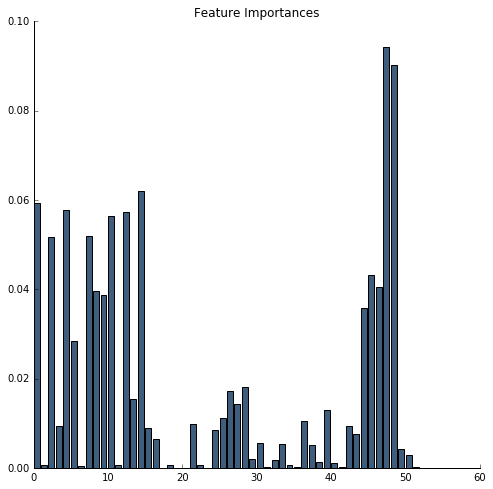
\includegraphics[scale=0.45]{report1.png}

\newcommand{\vh}{\mathbf{h}}

\section{Model Description}
We begin our investigation by testing our favorite classifiers, SVM and SGD. However, they did not perform very well in this dataset (80\% vs 76\%) and the class benchmark is 90\%. On the second look at the dataset description and our feature design, we find out why. Firstly, we use label encoder to encode categorical variables, and so we have removed concept of distance from the most important features of the data. Secondly, most of feaures deal with some sorts of syntatic structures which are rule-based by nature. As such, we suspect that non-linear classifier like decision tree or ensemble of trees may perform best. \\ \\
In the proceeding, we will discuss in length about multiple classifiers we use to achieve great performance. As expected, the ensemble of trees accomplish superior performance($> 94$\%). In order to boost our score further, we take the concept of ensembling to the extreme by employing a variation of ensemble blending popularized in Netflix Grand Prize competition.

\subsection{K Nearest Neighbors}
The KNN algorithm tries to directly approximate the decision boundaries of $f^*$. It computes the $k$ training points that are closest to $x$ based on Euclidean distance and return the purality of the labels of these $k$ points as the label of $x$.

\subsection{Decision Tree}
The decision tree algorithm create a decision function \(f: \mathcal{X}\rightarrow\mathcal{Y}\) represented by a binary tree. In every node, it picks the rule $h$ that maximally reduces uncertainty.
\begin{equation}
h = \argmax_h (u(s)-(p_L \cdot u(S_L) + p_R \cdot u(S_R)))
\end{equation} 
The uncertainty we in this competition are:
\begin{enumerate}
\item Classification error:
\begin{equation}
u(S)=1-\max_{k \in \mathcal{Y}} p_k^2
\end{equation} 
\item Gini index:
\begin{equation}
u(S)=1-\sum_{k \in \mathcal{Y}} p_k^2
\end{equation} 
\end{enumerate}

\subsection{Random Forest}
% http://www.math.usu.edu/adele/RandomForests/Ovronnaz.pdf
Random Forest is a kind of boosting algorithm, which combines a lot of weak classifiers(decision tree) and vote/average these trees to get the predication result.
\begin{enumerate}
\item it grows each tree with N independently sampled points with replacement from the training data.
\item At each node:
\begin{enumerate}
\item It randomly select $S$ features out of all possible features.
\item Find the rule that maximally reduces uncertainty on the selected $m$ features.
\end{enumerate}
\item It vote/average the predictions of all the trees to get the final prediction.
\end{enumerate}

\subsection{Extra tree}
Extra trees algorithm is a variance of random forest. The difference is that random forest choosing the most discriminative thresholds from the random subset of candidate features, while extra trees randomly select some thresholds and choose pick the best one as the splitting rule.

\subsection{Gradient Tree Boosting}
% http://scikit-learn.org/stable/modules/ensemble.html
The algorithm is an additive models with the following form
\begin{equation}
F_m(x)=\sum_{m=1}^{M}\gamma_m h_m(x)
\end{equation}
where $h_m(x)$ is the weak classifier which is a fixed-size decision tree for the Gradient Tree Boosting algorithm. \\
At each stage the we choose a decision tree $h_m(x)$that minimize the loos function $L$ given the current model $F_{m-1}$:  
\begin{equation}
F_m(x)=F_{m-1}+\gamma_m \argmin_h\sum_{i=1}^n L(y_i,F_{m-1}(x_i)-h(x))
\end{equation}
\indent Thus, we can solve the minimization problem by using gradient descent and the steepest descent direction is the negative gradient of the loss function:
\begin{equation}
F_m(x)=F_{m-1}+\gamma_m \sum_{i=1}^n \triangledown_F L(y_i,F_{m-1}(x_i))
\end{equation}
Where the step length $\gamma_m$ is 
\begin{equation}
\gamma_m=\argmin_{\gamma}\sum_{i=1}^n(\triangledown_F L(y_i,F_{m-1}(x_i))-\gamma\frac{\partial L(y_i,F_{m-1}(x_i))}{\partial F_{m-1}(x_i)}) 
\end{equation}

\subsection{Adaboost}
The core idea of Adaboost algorithm is to learn a lot of weak classifiers aw subset of the data. Then we assign a weight to each classifier and combine the weighted majority vote to produce the final prediction. \\
For this competition, we choose random forest and extra trees to be the "weak" classifier of Adaboost. 

\subsection{3-Layer Ensemble Blending}
As mentioned in previous subsections, algorithms which employ ensemble mechanism such boosting or bagging perform really well. However, they all seem to hit a plateau around $94.5\%$ accuracy score. Similar to boosting technique, an intuitive idea is to find a way to make these great performers to work together in hope of achieving stellar score. \\ \\
Inspired by blending algorithms popularized by Netflix competition and Neural Network, we introduce 3-layer blending algorithm.
\\
\begin{itemize}
\item \textbf{Layer 1: Online training} In this layer, we collect an ensemble of high achievers consisting of 2 random forest classifiers, 2 extra tree classifiers, one gradient boosting machine classifier, one AdaBoost of random forest, one AdaBoost of extra tree classifier, one bagging classifier of random forest, one bagging classifier of extra tree classifier, one bagging classifier of a simple decision tree, 2 decision tree classifiers and 3 kNN classifiers. Each is trained over the dataset multiple times by using 5-fold cross validation and output the average of probablistic predictions. Then, their results are combined together as a new dataset where each column feature representing one particular model mean probabilistic guesses and each row is an data example.
\item \textbf{Layer 2: Online Logistic Regression} inspired by Neural Network structure, we use logistic regression in the 2nd layer to regress layer 1 probablistic guesses into the final answers. We compute the 3-fold cross validation score and save output to a file.
\item \textbf{Layer 3: Offline aggregating} Over the course of the competition, we have trained literally dozen of models, some have very high cross validation score. By choosing only one best model, we lose most of our efforts doing extensive model experimentation in last couple of weeks and be unfair to marginally worse models. As such, we come up with offline hard voting scheme where we load all quiz prediction files with high internal cross validation score and aggregate them all together by using majority voting scheme.
\end{itemize}


\section{Model Selection}
To select the best parameters, we uses 3-fold cross validation. The k-fold cross validation procedure is as followed:
\begin{enumerate}
\item Splited the data into K parts.
\item For each value of \(\vh\): 
\begin{itemize}
\item For each \(k \in {1,2,\dots,K}\)
\begin{enumerate}
\item Train classifier \(\hat{f}_{\vh,k}\) using all $S_i$ except $S_k$.
\item Evaluate classifier \(\hat{f}_{\vh,k}\) using $S_k$: err(\(\hat{f}_{\vh,k}\),$S_k$)
\end{enumerate}
\item Cross-validation error for $\vh$: \(\frac{1}{K}\sum_{k=1}^K\) err\((\hat{f}_{\vh,k},S_k)\)
\end{itemize}
\item Select the value \(\hat{\vh}\) with lowest cross-validation error.
\end{enumerate}
\indent Cross validation is used to tune the parameters for each algorithms listed above. Then we choose the models with the fair performance and feed them into the blending algorithm to see if they contribute to the final result. At last, we choose a combination of model that produce the best result. 

\section{Predictor Evaluation}
In the begining, we tend to base our algorithm decision on the Kaggle Public Leaderboard score. However, we quickly realize that it is not a good idea. By doing so, we are exposed ourselves to chance of overfiitng the public leaderboard and spend unproductive time twisting parameters to gain minimal gain. \\ \\
Gradually, we learn to trust our local cross validation procedure, by using sklearn GridSearchCV to tune paremeters, we are able to combine the task of tuning parameters with the quest of searching for a high cross validation score. We discover that there is a high correlation between hiking local cross validation score and boosting public leaderboard score.

\section{Result of evaluation and analysis}
By spending many hours exploring and experiment, we are able to come up with the 3-layer algorithm discussed in \textbf{Model Description}. The algorithm is able to accomplish 95.667\% accuracy in the Kaggle Public Leaderboard and attain around 95.27\% local 3-fold cross validation score. As you can see there is a slight disprepancy between local cv score and leaderboard score. This reflects our bias of trying to submit the results that increases the leaderboard ranking. However, the disprepancy is small enough to be negligible.
% conference papers do not normally have an appendix


% use section* for acknowledgment
\section*{Acknowledgment}
We would like to thank the instructor Satyen Kale and COMS4771 teaching staff for putting together a well thought competition to stimulate us to apply machine learning theory into practice.





% trigger a \newpage just before the given reference
% number - used to balance the columns on the last page
% adjust value as needed - may need to be readjusted if
% the document is modified later
%\IEEEtriggeratref{8}
% The "triggered" command can be changed if desired:
%\IEEEtriggercmd{\enlargethispage{-5in}}

% references section

% can use a bibliography generated by BibTeX as a .bbl file
% BibTeX documentation can be easily obtained at:
% http://mirror.ctan.org/biblio/bibtex/contrib/doc/
% The IEEEtran BibTeX style support page is at:
% http://www.michaelshell.org/tex/ieeetran/bibtex/
%\bibliographystyle{IEEEtran}
% argument is your BibTeX string definitions and bibliography database(s)
%\bibliography{IEEEabrv,../bib/paper}
%
% <OR> manually copy in the resultant .bbl file
% set second argument of \begin to the number of references
% (used to reserve space for the reference number labels box)
\begin{thebibliography}{1}

\bibitem{IEEEhowto:kopka}
H.~Kopka and P.~W. Daly, \emph{A Guide to \LaTeX}, 3rd~ed.\hskip 1em plus
  0.5em minus 0.4em\relax Harlow, England: Addison-Wesley, 1999.
\bibitem{IEEEhowto:kopka}
Andreas Taoscher and Michael Jahrer , The Big Chaos Solution to the Netfix Grand Prize“ 
\end{thebibliography}



% that's all folks
\end{document}


